% ============================================================
% NodeAlert IoT — Artículo Científico
% Formato: APA 7.ª edición | Compilador: pdfLaTeX + Biber
% Compilar con:
%   pdflatex main.tex
%   biber main
%   pdflatex main.tex
%   pdflatex main.tex
% ============================================================
\documentclass[11pt, a4paper]{article}

% ---- Codificación y lenguaje ----
\usepackage[utf8]{inputenc}
\usepackage[T1]{fontenc}
\usepackage[spanish, es-nodecimaldot]{babel}

% ---- Tipografía: Arial (helvética como sustituto en LaTeX) ----
\usepackage{helvet}
\renewcommand{\familydefault}{\sfdefault}

% ---- Márgenes APA 7: laterales 3 cm, sup/inf 2.5 cm ----
\usepackage[
  top=2.5cm,
  bottom=2.5cm,
  left=3cm,
  right=3cm,
  headheight=15pt
]{geometry}

% ---- Interlineado APA (doble) ----
\usepackage{setspace}
\doublespacing

% ---- Ajuste de interlineado en tablas, figuras y código ----
\usepackage{etoolbox}
\AtBeginEnvironment{table}{\singlespacing}
\AtBeginEnvironment{figure}{\singlespacing}
\AtBeginEnvironment{lstlisting}{\singlespacing}

% ---- Encabezado y pie de página ----
\usepackage{fancyhdr}
\pagestyle{fancy}
\fancyhf{}
\fancyhead[R]{\thepage}
\fancyhead[L]{\small\textit{NODEALERT IoT --- PALAVECINO, KIROV, ALEMANDI}}
\renewcommand{\headrulewidth}{0pt}

% ---- Matemáticas ----
\usepackage{amsmath, amssymb}

% ---- Gráficos y color ----
\usepackage{graphicx}
\usepackage[dvipsnames, table]{xcolor}
\usepackage{float}

% ---- Tablas ----
\usepackage{booktabs}
\usepackage{multirow}
\usepackage{array}
\usepackage{tabularx}
\usepackage{longtable}

% ---- Listas ----
\usepackage{enumitem}
\setlist[itemize]{noitemsep, topsep=4pt}
\setlist[enumerate]{noitemsep, topsep=4pt}

% ---- Código fuente ----
\usepackage{listings}
\lstset{
  basicstyle=\small\ttfamily,
  breaklines=true,
  frame=single,
  captionpos=b,
  numbers=left,
  numberstyle=\tiny,
  keywordstyle=\bfseries,
  commentstyle=\itshape,
  showstringspaces=false
}

% ---- Comillas tipográficas (requerido por biblatex con babel) ----
\usepackage{csquotes}

% ---- Hipervínculos ----
\usepackage[
  colorlinks=true,
  linkcolor=black,
  citecolor=black,
  urlcolor=blue,
  hidelinks
]{hyperref}

% ---- Bibliografía APA 7 con biblatex-apa ----
\usepackage[
  backend=biber,
  style=apa,
  sortcites=true,
  sorting=nyt
]{biblatex}
\addbibresource{referencias.bib}

% ---- TikZ para diagramas ----
\usepackage{tikz}
\usetikzlibrary{shapes.geometric, arrows.meta, positioning, fit, backgrounds}

% ---- Captions APA ----
\usepackage{caption}
\captionsetup{
  font=small,
  labelfont=bf,
  justification=raggedright,
  singlelinecheck=false
}

% ---- Párrafos: sangría y espaciado ----
\setlength{\parindent}{0.5in}   % APA: sangría de primera línea
\setlength{\parskip}{0pt}

% ---- Sección sin numeración para abstract ----
\newcommand{\abstractsection}[1]{%
  \vspace{6pt}
  \noindent\textbf{#1}
  \vspace{2pt}
}

% ---- Numeración de ecuaciones ----
\numberwithin{equation}{section}

% ============================================================
%                   DOCUMENTO
% ============================================================
\begin{document}

% ---- Portada / Cabecera del artículo ----
\begin{center}
  {\large\bfseries
    NodeAlert IoT: Sistema Embebido de Monitoreo Ambiental
    y Control Autónomo de Iluminación basado en MQTT
    para Entornos Educativos\par}

  \vspace{18pt}

  {\normalsize\bfseries
    Palavecino, Sebastián\textsuperscript{1} \quad
    Kirov, Eloy\textsuperscript{1} \quad
    Alemandi, Francisco\textsuperscript{1}
    \par}

  \vspace{6pt}
  {\small\itshape
    \textsuperscript{1}Carrera de Ingeniería en Computación,\\
    Universidad Nacional de Rafaela (UNRaf), Rafaela, Santa Fe, Argentina\par}

  \vspace{6pt}
  {\small
    Cátedra: Ingeniería en Computación II\par
    Docentes a cargo: Milton Pozzo y Matías Wanzenried\par}
\end{center}

\vspace{12pt}
\hrule
\vspace{12pt}

% ---- Resumen, Palabras Clave, Abstract, Keywords ----
% ============================================================
% 01_resumen.tex — Resumen, Palabras clave, Abstract, Keywords
% ============================================================

\abstractsection{Resumen}

\noindent
El presente trabajo describe el diseño, desarrollo e implementación de NodeAlert IoT,
un sistema embebido de monitoreo ambiental y control autónomo de iluminación orientado
a entornos educativos. El sistema integra un microcontrolador ESP32-C3 programado bajo
ESP-IDF con FreeRTOS, tres sensores conectados por bus \(I^2C\) —dos fotosensores BH1750
y un sensor de temperatura/humedad SHT30—, y un sensor de presencia por radar de
microondas HLK-LD2420 interfaceado por UART. La lógica de control de iluminación
opera de forma completamente autónoma en el firmware, con histéresis de doble umbral
y un antirebote por software de 2\,s, sin depender de conectividad de red. La
telemetría se publica mediante el protocolo MQTT hacia un servidor Mosquitto
desplegado en un contenedor Docker sobre Raspberry Pi. El backend de procesamiento
se implementó en Node-RED con almacenamiento persistente en SQLite y expone una API
REST que alimenta un frontend web desarrollado en React. El sistema satisface los
requisitos mínimos de la cátedra: programación de microcontrolador,
comunicación bidireccional vía MQTT, broker propio
configurado con autenticación, publicadores y suscriptores diferenciados, e interfaz
de usuario con visualización de variables y controles remotos. El prototipo fue
validado en condiciones de laboratorio demostrando operación autónoma estable y
correcta integración de todos los subsistemas.

\vspace{10pt}
\noindent\textbf{Palabras clave:} Internet de las Cosas, ESP32-C3, MQTT, Node-RED,
control de iluminación, sensor de presencia, BH1750, SHT30, LD2420, Docker.

\vspace{20pt}
\hrule
\vspace{10pt}

\abstractsection{Abstract}

\noindent
This paper describes the design, development, and implementation of NodeAlert IoT,
an embedded environmental monitoring and autonomous lighting control system aimed
at educational environments. The system integrates an ESP32-C3 microcontroller
programmed under ESP-IDF with FreeRTOS, three sensors connected via \(I^2C\) bus
—two BH1750 light sensors and an SHT30 temperature/humidity sensor—, and an
HLK-LD2420 microwave radar presence sensor interfaced over UART. The lighting
control logic operates fully autonomously within the firmware, featuring dual-threshold
hysteresis and a 2\,s software debounce, independently of network connectivity.
Telemetry is published over MQTT to a Mosquitto broker running in a Docker container
on a Raspberry Pi. The processing backend is implemented in Node-RED with SQLite
persistent storage and exposes a REST API that feeds a React-based web frontend.
The system fulfills the course's minimum requirements: microcontroller programming,
bidirectional MQTT communication, a self-configured
authenticated broker, differentiated publishers and subscribers, and a user interface
with variable visualization and remote controls. The prototype was validated under
laboratory conditions, demonstrating stable autonomous operation and correct
integration of all subsystems.

\vspace{10pt}
\noindent\textbf{Keywords:} Internet of Things, ESP32-C3, MQTT, Node-RED,
lighting control, presence sensor, BH1750, SHT30, LD2420, Docker.

\vspace{10pt}
\hrule



\clearpage

% ---- Cuerpo del artículo ----
% ============================================================
% 02_introduccion.tex
% ============================================================

\section{Introducción}

La gestión eficiente de los recursos energéticos en edificios educativos representa
uno de los desafíos centrales del paradigma de Edificios Inteligentes (\textit{Smart
Buildings}). Según datos de la Agencia Internacional de Energía, el sector de
edificaciones es responsable de aproximadamente el 30\,\% del consumo energético
mundial, y la iluminación artificial constituye una fracción significativa de dicho
consumo en ambientes de uso discontinuo como aulas universitarias \parencite{IEA2023}.
En estos espacios, la iluminación permanece frecuentemente encendida en ausencia
de ocupantes o cuando el nivel de luz natural resulta suficiente, lo que genera un
desperdicio energético evitable.

Los sistemas de control inteligente de iluminación han demostrado reducciones de
consumo del orden del 30\,\% al 60\,\% respecto a instalaciones convencionales
\parencite{Kralikova2016}. Sin embargo, las soluciones comerciales disponibles
presentan elevados costos de adquisición e instalación, escasa flexibilidad para
entornos de investigación y, en la mayoría de los casos, dependencia de plataformas
propietarias que dificultan su estudio y modificación.

El surgimiento de microcontroladores de bajo costo con conectividad Wi-Fi integrada
—en particular la familia ESP32 de Espressif Systems— y de plataformas IoT de código
abierto como Node-RED, han abierto la posibilidad de construir sistemas de monitoreo
y control ambiental de bajo costo, alta adaptabilidad y arquitectura abierta
\parencite{NodeRED2024, Espressif2024}. El protocolo MQTT (\textit{Message Queuing
Telemetry Transport}), diseñado originalmente por IBM para redes de baja latencia y
ancho de banda reducido, se ha consolidado como el estándar de facto para la
comunicación entre dispositivos IoT \parencite{Banks2019}.

En este contexto, el presente trabajo describe el diseño, desarrollo e implementación
de \textbf{NodeAlert IoT}, un sistema prototipo que integra:

\begin{enumerate}[label=(\roman*)]
  \item Un nodo sensor embebido basado en ESP32-C3 que mide luminosidad,
        temperatura, humedad y detecta presencia de personas mediante radar
        de microondas, aplicando una lógica local de control de iluminación
        independiente de la conectividad de red;
  \item Un servidor central desplegado sobre Raspberry Pi mediante contenedores
        Docker, que implementa un broker MQTT Mosquitto, un motor de flujos
        Node-RED con almacenamiento SQLite y una API REST;
  \item Una interfaz web desarrollada en React que permite visualizar en tiempo
        real el estado de los nodos y enviar comandos remotos.
\end{enumerate}

El trabajo forma parte del Trabajo Final de la materia Ingeniería en Computación II
de la Universidad Nacional de Rafaela (UNRaf), cuyos requisitos mínimos establecen: programación de microcontrolador con
lógica de muestreo y optimización de recursos, modos de ahorro de energía,
comunicación bidireccional por MQTT, configuración propia de broker de datos,
suscriptores y publicadores, e interfaz de usuario con visualización y controles
\parencite{CatedraICII2026}.

El artículo se organiza de la siguiente manera: la Sección~\ref{sec:marco} presenta
los fundamentos teóricos y antecedentes; la Sección~\ref{sec:materiales} detalla los
materiales y métodos; las Secciones~\ref{sec:arquitectura}
y~\ref{sec:desarrollo} describen el diseño e implementación del sistema; la
Sección~\ref{sec:resultados} presenta los resultados de validación; las
Secciones~\ref{sec:discusion} y~\ref{sec:conclusiones} ofrecen discusión y
conclusiones.


% ============================================================
% 03_marco_teorico.tex
% ============================================================

\section{Marco Teórico y Antecedentes}
\label{sec:marco}

\subsection{Internet de las Cosas (IoT) en entornos educativos}

El Internet de las Cosas (IoT, por sus siglas en inglés) se define como la red de
objetos físicos equipados con sensores, software y conectividad que les permite
intercambiar datos con otros sistemas y dispositivos \parencite{Atzori2010}. En el
ámbito de los edificios educativos, las aplicaciones IoT se han orientado
principalmente a la gestión energética, el monitoreo de calidad del aire, el control
de acceso y la automatización de la iluminación \parencite{Jia2019}.

\textcite{Shaikh2014} señalan que los sistemas de control de iluminación basados
en sensores de ocupación y luminosidad constituyen uno de los casos de uso IoT con
mayor retorno de inversión en entornos de uso esporádico como aulas universitarias.
La combinación de sensores fotoeléctricos y detectores de presencia permite aplicar
estrategias de control adaptativo que atienden simultáneamente al confort visual y
al ahorro energético.

\subsection{Protocolo MQTT}

MQTT es un protocolo de mensajería ligero basado en el modelo publicador/suscriptor
(\textit{publish/subscribe}). Un elemento central del protocolo es el
\textit{broker}, servidor que gestiona la distribución de mensajes entre clientes
según los temas (\textit{topics}) a los que están suscritos. MQTT opera sobre TCP/IP
y define tres niveles de calidad de servicio (QoS): entrega sin garantía (QoS\,0),
entrega al menos una vez (QoS\,1) y entrega exactamente una vez (QoS\,2)
\parencite{Banks2019}.

La versión 3.1.1 del estándar, publicada por OASIS, es la más ampliamente soportada
en hardware embebido. El cliente MQTT integrado en el ESP-IDF de Espressif
implementa dicha versión e incluye soporte para reconexión automática,
autenticación por usuario y contraseña, y publicaciones con retención
\parencite{Espressif2024}.

\subsection{ESP32-C3 y ESP-IDF}

El ESP32-C3 es un SoC (System-on-Chip) de Espressif Systems basado en la
arquitectura RISC-V de 32 bits, con Wi-Fi 802.11\,b/g/n y Bluetooth 5 (LE)
integrados. Opera a frecuencias de hasta 160\,MHz y dispone de 400\,KB de SRAM y
4\,MB de Flash \parencite{EspressifDS2024}. Para aplicaciones IoT de bajo consumo,
el chip implementa modos \textit{modem sleep}, \textit{light sleep} y
\textit{deep sleep}, con consumos de tan solo 5\,µA en el modo más profundo.

El ESP-IDF (\textit{Espressif IoT Development Framework}) es el framework oficial de
desarrollo para la familia ESP32. Proporciona una capa de abstracción de hardware
(HAL) sobre FreeRTOS, drivers certificados para periféricos —incluyendo I\textsuperscript{2}C
maestro, UART y Wi-Fi—, y un sistema de gestión de componentes que facilita la
incorporación de bibliotecas externas como cJSON y el cliente MQTT
\parencite{Espressif2024}.

\subsection{Sensores utilizados}

\subsubsection{BH1750 — Sensor de luminancia}

El BH1750FVI es un sensor digital de luminancia ambiental de 16 bits fabricado por
Rohm Semiconductor, con interfaz I\textsuperscript{2}C. Opera en el rango de 1 a
65535\,lx con resolución de 1\,lx en modo de alta resolución continua
(\textit{Continuous H-Resolution Mode}). Admite dos direcciones I\textsuperscript{2}C
(0x23 y 0x5C) según el estado del pin ADDR, lo que posibilita la conexión de dos
unidades en el mismo bus \parencite{Rohm2011}.

La conversión analógica-digital de la señal fotoeléctrica interna entrega un valor
crudo de 16 bits que se convierte a lux mediante la ecuación:

\begin{equation}
  E_v = \frac{V_{\text{raw}}}{1{,}2}
  \label{eq:bh1750}
\end{equation}

\noindent donde $E_v$ es la iluminancia en lux y $V_{\text{raw}}$ es el valor
entero de 16 bits leído del sensor.

\subsubsection{SHT30/SHT31 — Sensor de temperatura y humedad}

El SHT30 de Sensirion es un sensor digital de temperatura y humedad relativa con
interfaz I\textsuperscript{2}C. Ofrece precisión de ±0,3\,°C en temperatura
(rango $-$40\,°C a +125\,°C) y ±3\,\%\,HR en humedad \parencite{Sensirion2023}.
El protocolo de comunicación contempla un comando de disparo de medición de 16 bits
y la lectura de 6 bytes de respuesta que incluyen temperatura, humedad y bytes de
verificación CRC-8.

Las fórmulas de conversión de los valores crudos de 16 bits son:

\begin{equation}
  T\,[\mathrm{{}^{\circ}C}] = -45{,}0 + 175{,}0 \cdot \frac{V_T}{2^{16}-1}
  \label{eq:sht_temp}
\end{equation}

\begin{equation}
  HR\,[\%] = 100{,}0 \cdot \frac{V_H}{2^{16}-1}
  \label{eq:sht_hum}
\end{equation}

\noindent donde $V_T$ y $V_H$ son los valores crudos de temperatura y humedad,
respectivamente \parencite{Sensirion2023}.

\subsubsection{HLK-LD2420 — Radar de presencia}

El HLK-LD2420 de Hi-Link es un módulo de radar FMCW (\textit{Frequency-Modulated
Continuous Wave}) de 24\,GHz diseñado para detección de presencia humana. A
diferencia de los sensores PIR (infrarrojo pasivo), el radar FMCW detecta tanto
movimiento macroscópico como la microvibración respiratoria de personas estáticas
\parencite{HiLink2023}. Opera en el rango de 0 a 8\,m con resolución de 0,7\,m y
se comunica mediante UART a 115200 baudios.

En modo de reporte nativo simple (\textit{Native Simple Report Mode}), el módulo
emite tramas de texto con tres tipos de mensajes: \texttt{ON} (presencia detectada),
\texttt{OFF} (sin presencia) y \texttt{Range }\textit{d} (distancia al objeto en
centímetros). Este modo reduce la complejidad del procesamiento en el
microcontrolador respecto al modo de protocolo binario.

\subsection{Node-RED}

Node-RED es una herramienta de programación visual basada en flujos para aplicaciones
IoT, desarrollada originalmente por IBM y actualmente mantenida por la OpenJS
Foundation \parencite{NodeRED2024}. Permite construir aplicaciones conectando nodos
funcionales de forma gráfica, con soporte nativo para protocolos MQTT, HTTP y WebSocket.
Implementado sobre Node.js, su ejecución en Raspberry Pi dentro de contenedores Docker
simplifica el despliegue y la portabilidad del sistema.

\subsection{Antecedentes relevantes}

\textcite{Cardiel2012} propusieron una arquitectura de middleware orientada a SCADA
basada en el modelo de publicación/suscripción, conceptualmente similar a la empleada
en este trabajo, con separación entre la capa de adquisición de datos y la capa de
lógica de negocio. \textcite{Jia2019} describieron un sistema IoT para gestión
energética de edificios educativos usando sensores de ocupación e iluminación,
obteniendo reducciones de consumo superiores al 40\,\%. Estos antecedentes respaldan
la viabilidad del enfoque adoptado en NodeAlert IoT.

% ============================================================
% 04_materiales_metodos.tex
% ============================================================

\section{Materiales y Métodos}
\label{sec:materiales}

\subsection{Hardware del nodo sensor}

El nodo sensor se implementó sobre una placa ESP32-C3 SuperMini, formato compacto
con factor de forma de 22,52\,mm × 18\,mm, que integra el SoC ESP32-C3 de Espressif
junto con antena de cerámica y regulador de 3,3\,V. La selección de esta plataforma
se fundamentó en su soporte nativo para Wi-Fi 802.11\,b/g/n, el modo
gestión de energía básica del ESP-IDF, y el soporte
oficial del framework ESP-IDF en su versión 6.1.0.

Los sensores conectados al nodo se detallan en la Tabla~\ref{tab:sensores}.

\begin{table}[htbp]
  \caption{\textit{Sensores del nodo ESP32-C3 y sus características principales.}}
  \label{tab:sensores}
  \centering
  \small
  \begin{tabularx}{\textwidth}{@{}lllX@{}}
    \toprule
    \textbf{Sensor} & \textbf{Magnitud} & \textbf{Interfaz} & \textbf{Parámetros clave} \\
    \midrule
    BH1750FVI (×2) & Luminancia & I\textsuperscript{2}C & 1–65535\,lx; 1\,lx resolución; dir. 0x23 y 0x5C \\
    SHT30 & Temp./Humedad & I\textsuperscript{2}C & ±0,3\,°C; ±3\,\%\,HR; dir. 0x44 \\
    HLK-LD2420 & Presencia/Radar & UART & 24\,GHz FMCW; 0–8\,m; 115200 baudios \\
    \bottomrule
  \end{tabularx}
  \vspace{4pt}

  \noindent\textit{Nota.} Todos los dispositivos I\textsuperscript{2}C comparten el bus I2C0
  (SDA: GPIO4, SCL: GPIO5) del ESP32-C3. El radar LD2420 emplea UART1 (RX: GPIO7, TX: GPIO6).
\end{table}

Adicionalmente, el nodo incorpora un relé de estado sólido controlado desde el
GPIO0 (activo en nivel bajo) para la conmutación de la carga de iluminación, y un
LED de indicación de presencia en GPIO1 (activo en nivel alto).

\begin{table}[htbp]
  \centering
  \caption{\textit{Asignación de pines del ESP32-C3 en el prototipo NodeAlert IoT.}}
  \label{tab:pinout}
  \begin{tabularx}{\textwidth}{l X}
    \toprule
    \textbf{GPIO} & \textbf{Componente / Función} \\
    \midrule
    GPIO0 & Relé de iluminación (activo en nivel bajo) \\
    GPIO1 & LED de indicación de presencia (activo en nivel alto) \\
    GPIO4 & I\textsuperscript{2}C SDA (BH1750 ventana/aula, SHT30) \\
    GPIO5 & I\textsuperscript{2}C SCL (BH1750 ventana/aula, SHT30) \\
    GPIO6 & UART1 TX hacia LD2420 (RX del sensor) \\
    GPIO7 & UART1 RX desde LD2420 (TX del sensor) \\
    \bottomrule
  \end{tabularx}
\end{table}

\subsection{Plataforma de servidor}

El servidor central se desplegó sobre una Raspberry Pi con sistema operativo Linux,
utilizando Docker Compose para la orquestación de tres contenedores:

\begin{enumerate}
  \item \textbf{nodealert-mqtt}: basado en la imagen oficial de Eclipse Mosquitto,
        configurado con autenticación por usuario y contraseña, lista de control
        de acceso (ACL) y persistencia de datos en volumen local. Expone el puerto
        1883/TCP.
  \item \textbf{nodealert-nodered}: imagen \texttt{nodered/node-red:latest}
        con el paquete adicional \texttt{node-red-node-sqlite} instalado en la
        imagen Docker personalizada. Expone el puerto 1880/TCP. Depende del
        contenedor Mosquitto con verificación de salud (\textit{healthcheck}).
  \item \textbf{nodealert-frontend}: servidor Nginx que sirve el frontend React
        compilado con Vite. Expone el puerto 3001/TCP en el host.
\end{enumerate}

Los tres contenedores se comunican a través de la red interna Docker
\texttt{nodealert-net} (driver \texttt{bridge}).

\subsection{Herramientas de desarrollo}

El firmware se desarrolló íntegramente en lenguaje C utilizando el ESP-IDF v6.1.0
con el sistema de construcción CMake/Ninja. Los componentes externos incorporados
mediante el gestor de componentes de ESP-IDF fueron:
\begin{itemize}
  \item \texttt{espressif/cjson}: biblioteca de serialización/deserialización JSON
        utilizada para componer los mensajes de telemetría.
  \item \texttt{espressif/mqtt}: cliente MQTT basado en el protocolo MQTT 3.1.1.
\end{itemize}

Los drivers de los sensores (BH1750, SHT30, LD2420) fueron desarrollados
específicamente para este proyecto sobre los drivers de bajo nivel de ESP-IDF
(\texttt{i2c\_master} y \texttt{uart}), sin dependencias de bibliotecas de Arduino.

El frontend web se desarrolló con React 18 y React Router v6, utilizando Recharts
para la visualización de series temporales y Axios para la comunicación con la
API REST. La herramienta de construcción empleada fue Vite 5.

Los flujos de Node-RED fueron generados programáticamente mediante un script
JavaScript (\texttt{generate-flows.js}) que produce el archivo \texttt{flows.json},
garantizando consistencia y facilidad de mantenimiento.

\subsection{Metodología de desarrollo}

El sistema se desarrolló siguiendo un enfoque incremental por capas, comenzando por
el firmware del nodo sensor, continuando con la infraestructura del servidor y
finalizando con la interfaz de usuario. Cada capa fue probada de forma independiente
antes de integrarla con las adyacentes:

\begin{enumerate}
  \item \textbf{Fase 1 — Firmware base}: inicialización de periféricos I\textsuperscript{2}C
        y UART, lectura de sensores, implementación de lógica de control de relé.
  \item \textbf{Fase 2 — Conectividad}: implementación del módulo Wi-Fi y cliente MQTT,
        publicación de telemetría JSON, suscripción a tópico de comandos.
  \item \textbf{Fase 3 — Servidor}: despliegue de Mosquitto, configuración de autenticación
        y ACL, diseño de flujos Node-RED y esquema de base de datos SQLite.
  \item \textbf{Fase 4 — API y Frontend}: implementación de la API REST en Node-RED,
        desarrollo del frontend React con actualización periódica de datos.
  \item \textbf{Fase 5 — Integración y validación}: pruebas end-to-end del flujo completo
        desde el sensor hasta la interfaz web.
\end{enumerate}


% ============================================================
% 05_arquitectura.tex
% ============================================================

\section{Arquitectura y Diseño de la Solución}
\label{sec:arquitectura}

\subsection{Arquitectura general del sistema}

NodeAlert IoT adopta una arquitectura IoT de tres capas: capa de percepción
(nodo sensor embebido), capa de comunicación (red Wi-Fi y broker MQTT) y capa
de aplicación (backend Node-RED, base de datos SQLite y frontend web). La
Figura~\ref{fig:arquitectura} ilustra esta organización.

\begin{figure}[htbp]
  \centering
  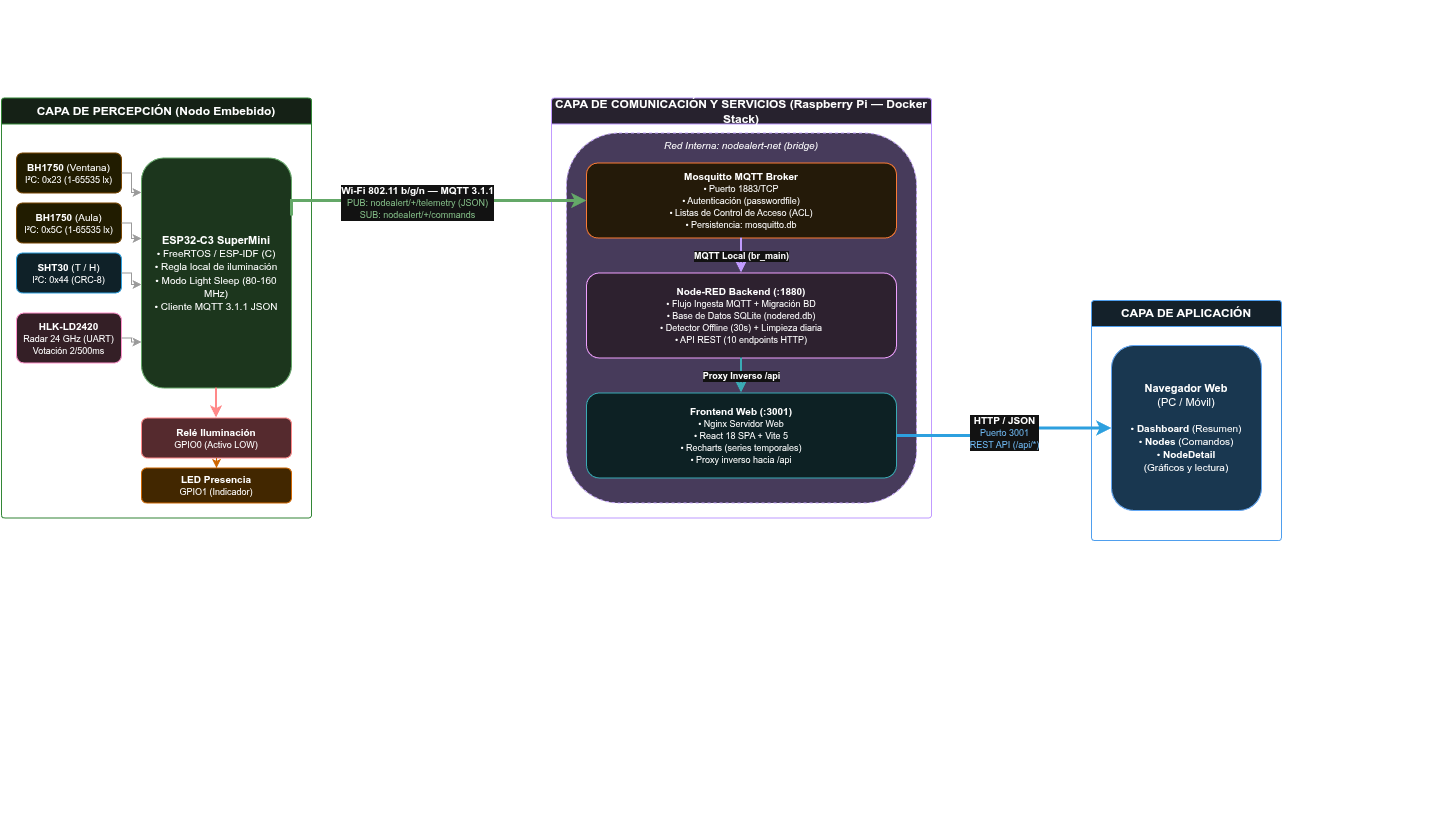
\includegraphics[width=0.95\textwidth]{figuras/arquitectura_general.png}
  \caption{\textit{Arquitectura general de NodeAlert IoT con sus tres capas: percepción, comunicación y aplicación.}}
  \label{fig:arquitectura}
\end{figure}

\subsection{Nodo sensor: arquitectura del firmware}

El firmware del nodo está diseñado en torno al bucle principal de la función
\texttt{app\_main}, que ejecuta en el contexto de la tarea principal de FreeRTOS.
La arquitectura evita la creación de tareas adicionales, manteniendo una única
tarea de ejecución que opera en un ciclo de 20\,ms. La Figura~\ref{fig:fw_bloques}
ilustra el diagrama de bloques del firmware.

\begin{figure}[htbp]
  \centering
  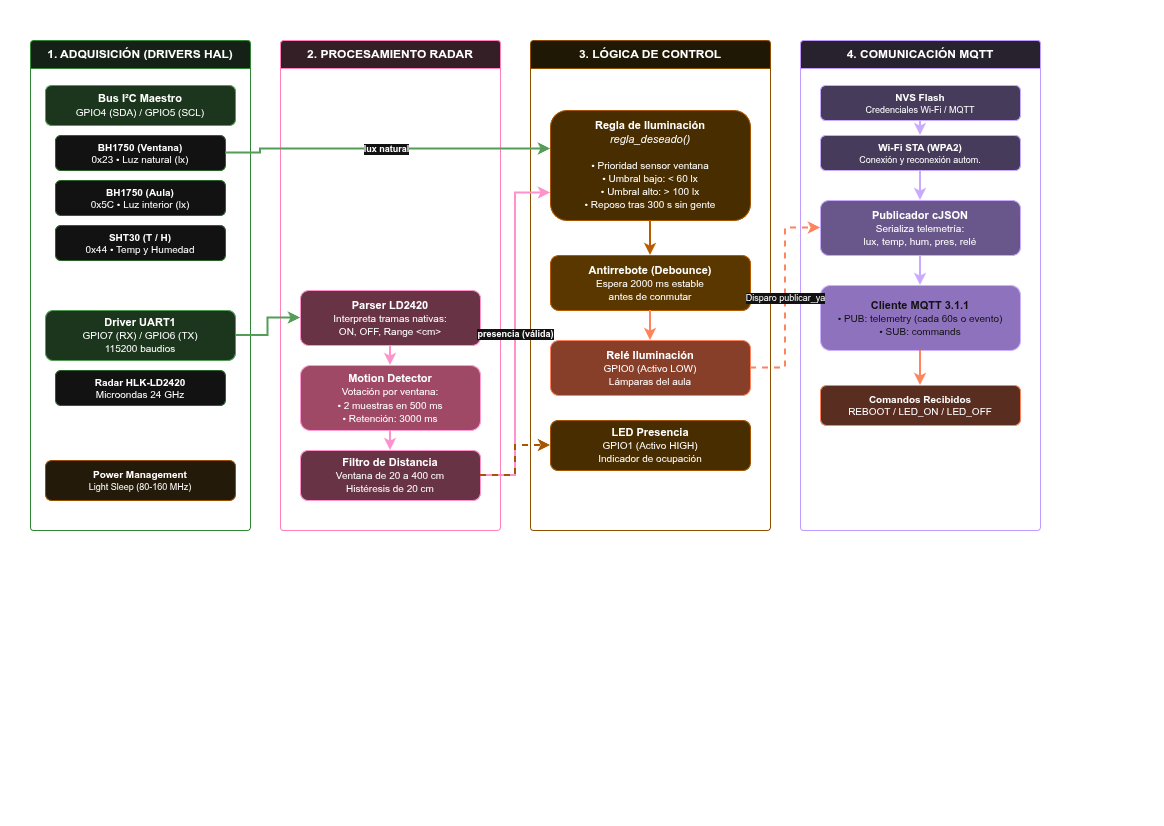
\includegraphics[width=0.95\textwidth]{figuras/firmware_bloques.png}
  \caption{\textit{Diagrama de bloques del firmware del nodo ESP32-C3.}}
  \label{fig:fw_bloques}
\end{figure}

\subsubsection{Módulo de sensores I\textsuperscript{2}C}

Los tres dispositivos I\textsuperscript{2}C (dos BH1750 y el SHT30) comparten el
bus I2C0 inicializado mediante el driver \texttt{i2c\_master} de ESP-IDF. Las
lecturas se realizan cada 1000\,ms. Cada driver implementa reconexión automática:
ante un fallo de comunicación, el dispositivo se marca como no disponible y se
reintenta la inicialización cada 30\,s. Esta estrategia de recuperación elástica
garantiza que la lógica de control continúe operando aunque uno o más sensores
fallen temporalmente.

\subsubsection{Módulo del radar LD2420}

El driver del radar LD2420 implementa en su totalidad el modo de reporte nativo
simple. Al inicializar, envía la secuencia de comandos binaria que configura el
módulo en este modo, con tramas delimitadas por los bytes \texttt{FD FC FB FA} y
\texttt{04 03 02 01}. El parser de líneas acumula los bytes UART en un buffer de
24 caracteres e interpreta los mensajes de texto emitidos.

Sobre el parser se ejecuta un detector de movimiento con lógica de votación que
requiere un mínimo de dos evidencias válidas en una ventana de 500\,ms para activar
la señal de presencia (\textit{required\_evidence} = 2,
\textit{evidence\_window} = 500\,ms). Una vez activada, la señal se mantiene
durante 3\,s adicionales sin nuevas evidencias (\textit{hold\_ms} = 3000). El
estado se declara obsoleto (\textit{stale}) si no se reciben datos en más de 1\,s.

\subsubsection{Lógica de control de iluminación}

La función de control de iluminación se implementó como una función pura sin
efectos secundarios en el archivo \texttt{regla\_luz.h}, siguiendo el principio
de separación entre lógica y hardware. La función \texttt{regla\_deseado()} recibe
como parámetros el estado actual del sistema, la disponibilidad y valores de los
sensores de luz, el estado actual del relé y los umbrales de iluminación, y
devuelve el estado deseado del relé.

La Figura~\ref{fig:diagrama_regla} ilustra el diagrama de flujo de la lógica de
control.

\begin{figure}[htbp]
  \centering
  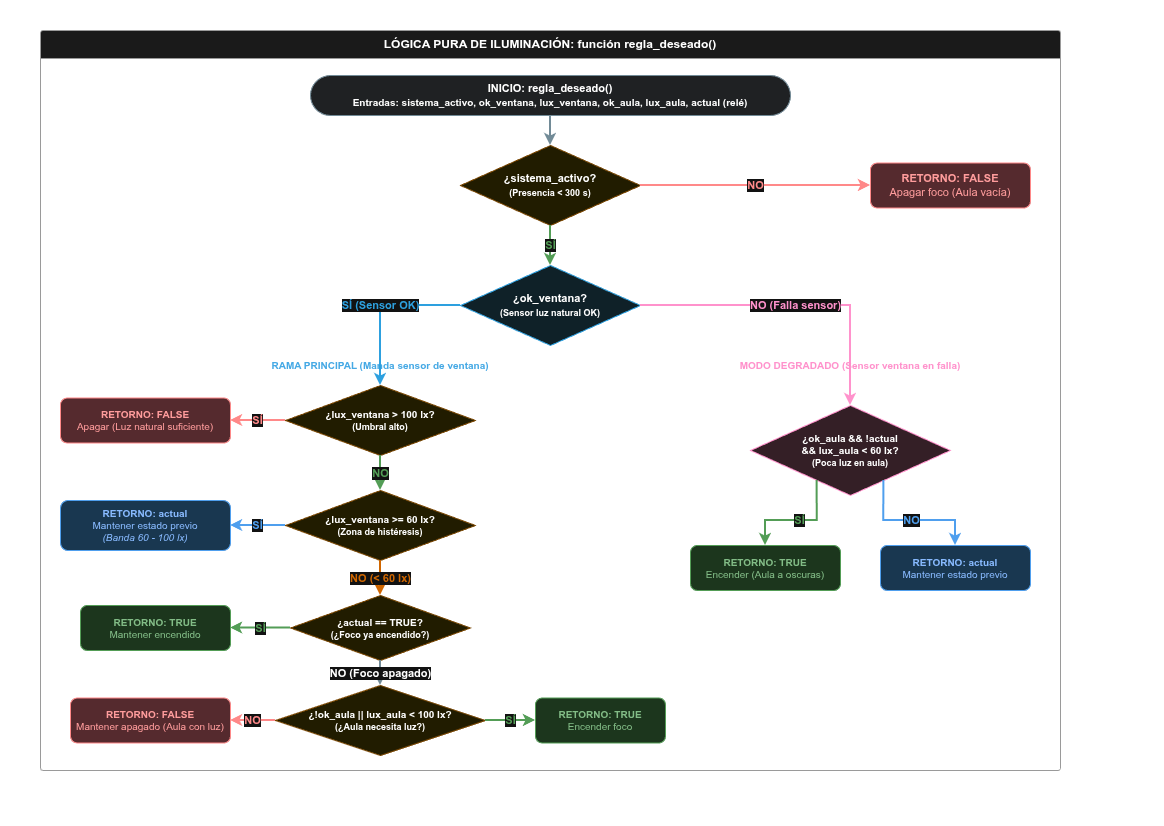
\includegraphics[width=0.88\textwidth]{figuras/diagrama_flujo_regla.png}
  \caption{\textit{Diagrama de flujo de la función \texttt{regla\_deseado()}: lógica de control de iluminación con histéresis de doble umbral.}}
  \label{fig:diagrama_regla}
\end{figure}

El debounce por software de 2\,s actúa en la capa de control del relé
(\texttt{controlar\_rele()}): un cambio de estado del relé solo se ejecuta si el
estado deseado se mantiene estable durante al menos 2000\,ms, evitando oscilaciones
ante variaciones bruscas de luminosidad.

\subsection{Arquitectura del servidor}

La Figura~\ref{fig:docker_arch} muestra la arquitectura de contenedores Docker.

\begin{figure}[htbp]
  \centering
  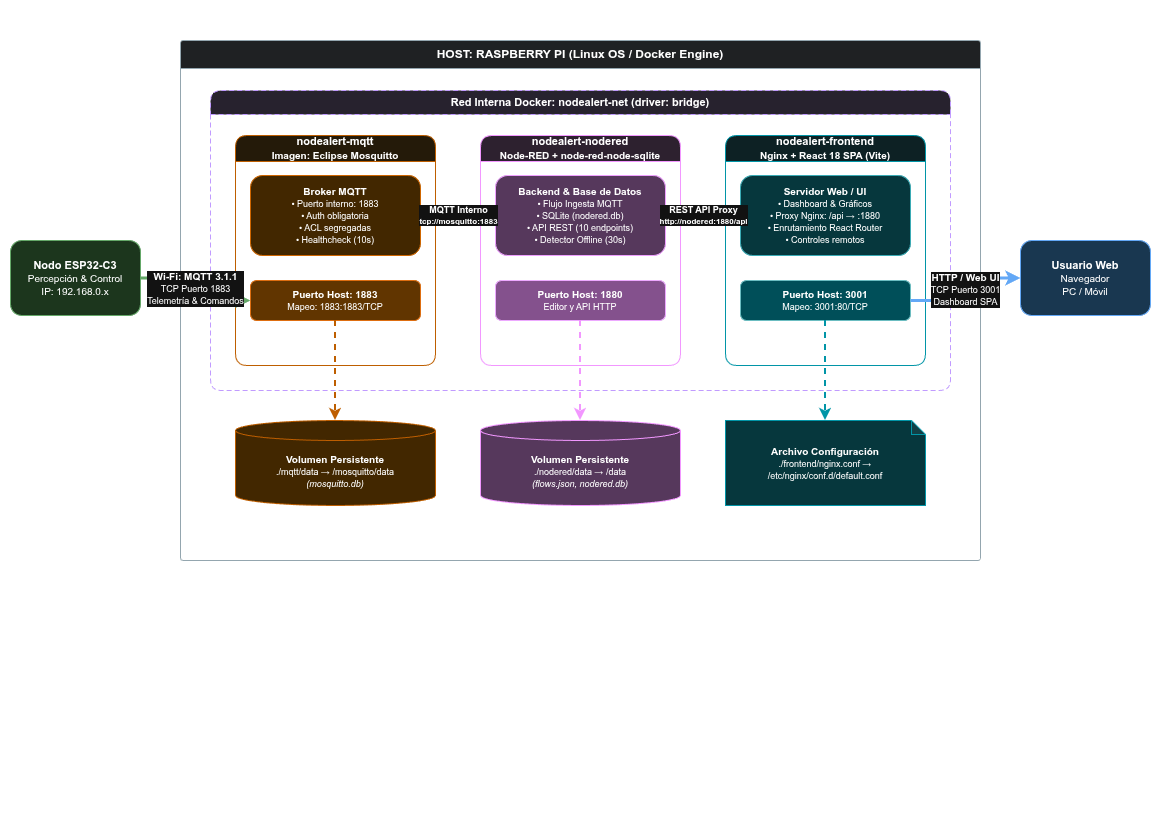
\includegraphics[width=0.95\textwidth]{figuras/docker_arquitectura.png}
  \caption{\textit{Arquitectura de contenedores Docker desplegada en Raspberry Pi. Los tres servicios se comunican a través de la red interna \texttt{nodealert-net}.}}
  \label{fig:docker_arch}
\end{figure}

\subsubsection{Esquema de base de datos SQLite}

Node-RED persiste todos los datos de telemetría en una base de datos SQLite local
(\texttt{nodered.db}). El esquema comprende tres tablas principales:

\begin{itemize}
  \item \textbf{nodes}: registro de nodos conocidos con campos \texttt{node\_id}
        (PK), \texttt{name}, \texttt{is\_online}, \texttt{last\_seen} y
        \texttt{hidden}.
  \item \textbf{telemetry}: serie temporal de mediciones con campos para
        temperatura, gas, llama, estado de presencia, iluminancia ventana/aula,
        temperatura interna, humedad y estado del relé, con índice sobre
        (\texttt{node\_id}, \texttt{timestamp}).
  \item \textbf{node\_config}: configuración por nodo (umbrales de temperatura,
        gas, llama) con valores predeterminados.
\end{itemize}

La tabla \texttt{telemetry} implementa un mecanismo de migraciones en cadena
ejecutado en el flujo \textit{Init DB} de Node-RED, que verifica la existencia de
cada columna antes de agregarla mediante \texttt{ALTER TABLE}, garantizando
compatibilidad hacia adelante.

\subsection{Tópicos MQTT}

La comunicación MQTT utiliza el espacio de nombres jerárquico
\texttt{nodealert/<device\_id>/\{telemetry | commands\}}, donde
\texttt{<device\_id>} es el identificador único del nodo (por ejemplo,
\texttt{nodealert-luz01}). La Tabla~\ref{tab:mqtt_topics} resume los tópicos
utilizados.

\begin{table}[htbp]
  \caption{\textit{Tópicos MQTT del sistema NodeAlert IoT.}}
  \label{tab:mqtt_topics}
  \centering
  \small
  \begin{tabularx}{\textwidth}{@{}llX@{}}
    \toprule
    \textbf{Tópico} & \textbf{QoS} & \textbf{Descripción} \\
    \midrule
    \texttt{nodealert/+/telemetry} & 1 & Telemetría JSON publicada por el nodo cada 60\,s o ante evento \\
    \texttt{nodealert/<id>/commands} & 1 & Comandos de texto enviados desde el servidor al nodo \\
    \bottomrule
  \end{tabularx}
  \vspace{4pt}

  \noindent\textit{Nota.} El símbolo \texttt{+} en el tópico de suscripción de Node-RED es
  un comodín de un nivel que permite recibir telemetría de todos los nodos registrados.
\end{table}

\subsection{API REST}

Node-RED expone una API REST HTTP sobre el puerto 1880 que el frontend React consume
mediante solicitudes Axios. La Tabla~\ref{tab:api_endpoints} lista los endpoints
implementados.

\begin{table}[htbp]
  \caption{\textit{Endpoints de la API REST expuesta por Node-RED.}}
  \label{tab:api_endpoints}
  \centering
  \small
  \begin{tabularx}{\textwidth}{@{}llX@{}}
    \toprule
    \textbf{Método} & \textbf{Endpoint} & \textbf{Descripción} \\
    \midrule
    GET  & \texttt{/api/health}                     & Estado del servicio \\
    GET  & \texttt{/api/nodes}                      & Lista de nodos visibles \\
    GET  & \texttt{/api/nodes/:id}                  & Detalle de nodo con última telemetría \\
    POST & \texttt{/api/nodes}                      & Registrar nodo manualmente \\
    DELETE & \texttt{/api/nodes/:id}                & Ocultar nodo (soft delete) \\
    GET  & \texttt{/api/telemetry/latest}           & Última telemetría de todos los nodos \\
    GET  & \texttt{/api/telemetry/:id}              & Historial de telemetría de un nodo \\
    GET  & \texttt{/api/telemetry/averages}         & Promedios de la última hora \\
    GET  & \texttt{/api/nodes/:id/config}           & Configuración del nodo \\
    POST & \texttt{/api/nodes/:id/command}          & Publicar comando vía MQTT \\
    \bottomrule
  \end{tabularx}
  \vspace{4pt}

  \noindent\textit{Nota.} El endpoint \texttt{POST /api/nodes/:id/config} devuelve
  HTTP 405, dado que los umbrales operativos son parámetros de compilación del firmware.
\end{table}


% ============================================================
% 06_desarrollo.tex
% ============================================================

\section{Desarrollo e Implementación}
\label{sec:desarrollo}

\subsection{Firmware del nodo ESP32-C3}

\subsubsection{Inicialización y configuración de periféricos}

El punto de entrada del firmware es la función \texttt{app\_main()}, que sigue el
siguiente orden de inicialización: (i) inicialización del almacenamiento no volátil
(NVS Flash) para parámetros de Wi-Fi y MQTT; (ii) inicialización del módulo Wi-Fi
en modo estación (STA); (iii) configuración de GPIO de salida para el relé e
indicador LED; (iv) inicialización del bus I\textsuperscript{2}C maestro y conexión
de los tres sensores; (v) inicialización del módulo UART y el radar LD2420; (vi) inicialización del módulo MQTT.

No se implementó light sleep: el firmware prioriza el monitoreo en tiempo real y
evita la pérdida de datos del radar LD2420 por UART durante el sueño. El ahorro
de energía se limita al clock gating automático del ESP-IDF.

\subsubsection{Bucle principal y lógica temporal}

El bucle principal ejecuta a un ritmo de 20\,ms (\texttt{vTaskDelay(pdMS\_TO\_TICKS(20))}),
controlando tres temporizadores independientes:

\begin{itemize}
  \item \textbf{Lectura de sensores}: cada 1000\,ms se leen los tres sensores
        I\textsuperscript{2}C.
  \item \textbf{Publicación MQTT}: la telemetría se publica cada 60\,s o
        inmediatamente cuando ocurre un evento significativo (cambio de estado del
        relé o de presencia del sistema), mediante la bandera \texttt{publicar\_ya}.
  \item \textbf{Actualización del radar}: en cada iteración del bucle (cada 20\,ms)
        se llama a \texttt{ld2420\_update()} para vaciar el buffer UART y procesar
        las tramas del radar.
\end{itemize}

La función de tiempo \texttt{aura\_millis()} encapsula \texttt{esp\_timer\_get\_time()}
con conversión a milisegundos en entero sin signo de 32 bits, garantizando que las
comparaciones de tiempo funcionen correctamente ante el desbordamiento a 32 bits
(cada \raise.17ex\hbox{$\scriptstyle\mathtt{\sim}$}49,7 días).

\subsubsection{Formato de mensaje de telemetría}

Los mensajes de telemetría se serializan en formato JSON mediante la biblioteca
cJSON. Un mensaje típico publicado en el tópico
\texttt{nodealert/nodealert-luz01/telemetry} tiene la siguiente estructura:

\begin{lstlisting}[caption={Ejemplo de mensaje JSON de telemetría.}, label={lst:json_tele}]
{
  "device_id":     "nodealert-luz01",
  "presencia":     1,
  "luz_ventana_lx": 123.4,
  "luz_aula_lx":   87.5,
  "temp_c":        23.1,
  "humedad_pct":   58.3,
  "rele_canal1":   1
}
\end{lstlisting}

Los campos opcionales (aquellos correspondientes a sensores en falla) se omiten del
mensaje en lugar de publicarse como \texttt{null}, reduciendo el tamaño del payload.
Los valores numéricos se redondean a un decimal mediante la función
\texttt{redondear1()}.

\subsubsection{Recepción de comandos}

El nodo suscribe al tópico \texttt{nodealert/nodealert-luz01/commands} al conectarse
al broker. Los comandos aceptados son cadenas de texto simples:
\texttt{REBOOT} (reinicia el dispositivo mediante \texttt{esp\_restart()}),
\texttt{LED\_ON} y \texttt{LED\_OFF} (controlan el LED de indicación de presencia).

\subsubsection{Detección de presencia y ventana de distancia}

El sistema evalúa la presencia de personas dentro de una ventana de distancia
configurada entre \texttt{DIST\_MIN\_CM} = 20\,cm y \texttt{DIST\_MAX\_CM} = 400\,cm.
Se aplica una histéresis de \texttt{DIST\_HIST\_CM} = 20\,cm para evitar
oscilaciones en los bordes de la ventana. La señal de presencia válida exige que el
radar reporte movimiento (\texttt{ld2420\_movimiento()} = \texttt{true}) y que la
distancia reportada esté dentro de la ventana de interés.

Cuando se detecta presencia, se actualiza el marcador temporal
\texttt{ultima\_presencia\_ms}. El sistema permanece en estado \textit{activo}
mientras no transcurran más de \texttt{DELAY\_OFF\_DEFECTO\_S} = 300\,s (5\,minutos)
desde la última detección de presencia, momento en que el sistema pasa al estado
de \textit{reposo} y la luz se apaga.

\subsection{Backend en Node-RED}

Los flujos de Node-RED se agrupan en cinco pestañas (\textit{tabs}) lógicas con
responsabilidades claramente delimitadas:

\begin{enumerate}
  \item \textbf{Init DB}: flujo disparado una vez al inicio del contenedor mediante
        un nodo \textit{inject} con \texttt{once: true}. Ejecuta en cadena la
        creación de tablas SQLite y una secuencia de migraciones que agregan columnas
        nuevas a tablas existentes solo si no están presentes, usando consultas
        \texttt{PRAGMA table\_info()}.
  \item \textbf{Telemetry}: nodo \textit{mqtt in} suscrito al tópico
        \texttt{nodealert/+/telemetry} (QoS 2). El nodo función
        \textit{Process telemetry} extrae los campos del payload JSON y construye
        una consulta SQL en batch que: (a) inserta o actualiza el registro del nodo
        en la tabla \texttt{nodes}; (b) inserta la lectura en \texttt{telemetry}
        solo si el nodo no está marcado como oculto (\texttt{hidden = 0}).
  \item \textbf{Offline Detector}: nodo \textit{inject} con repetición cada 30\,s
        que consulta los nodos marcados como \textit{online} cuya última vista
        fue hace más de 60\,s y los marca como \textit{offline}.
  \item \textbf{Cleanup}: limpieza diaria (\textit{inject} con repetición de
        86400\,s) que elimina registros de telemetría con más de 30 días de
        antigüedad.
  \item \textbf{API}: diez endpoints HTTP implementados mediante pares de nodos
        \textit{http in} / \textit{http response}, con nodos función intermedios
        para construcción de consultas SQL y un nodo \textit{mqtt out} para el
        endpoint de comandos.
\end{enumerate}

\subsection{Frontend React}

La aplicación frontend se estructura en tres vistas principales accesibles desde
una barra lateral de navegación:

\begin{enumerate}
  \item \textbf{Dashboard}: muestra tarjetas resumen con la cantidad de nodos en
        línea, fuera de línea y total, seguidas de una tabla con la última lectura
        de cada nodo. Los datos se actualizan automáticamente cada 10\,s mediante
        \texttt{setInterval}.
  \item \textbf{Nodes}: lista tabular de todos los nodos con estado,
        última vista, controles de renombrado local (persistido en
        \texttt{localStorage}) y botones para enviar comandos individuales (Reboot,
        Buzzer ON/OFF) y eliminar nodos.
  \item \textbf{NodeDetail}: vista detallada de un nodo individual con tarjetas
        de estado actual para cada variable (temperatura, gas, llama, presencia,
        iluminancia ventana/aula, humedad, estado del relé) y gráficos de serie
        temporal mediante Recharts (últimas 50 lecturas, actualizados cada 10\,s).
\end{enumerate}

La comunicación con la API emplea la biblioteca Axios con la URL base \texttt{/api},
proxeada en desarrollo mediante Vite hacia \texttt{http://localhost:1880}.
En producción, Nginx está configurado para reenviar las solicitudes \texttt{/api}
al contenedor Node-RED.

La Figura~\ref{fig:frontend_dashboard} reserva el espacio para una captura de la
interfaz del Dashboard.

\begin{figure}[htbp]
  \centering
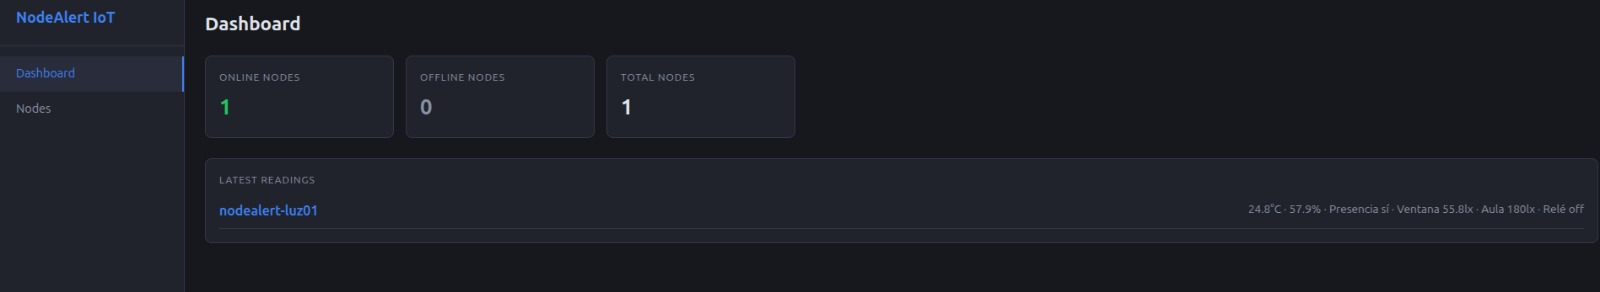
\includegraphics[width=0.95\textwidth]{figuras/dashb.jpeg}

  \caption{\textit{Interfaz principal (Dashboard) de la aplicación web NodeAlert IoT con resumen de nodos y últimas lecturas de telemetría.}}
  \label{fig:frontend_dashboard}
\end{figure}

La Figura~\ref{fig:frontend_detail} muestra el espacio reservado para la vista de
detalle de un nodo.

\begin{figure}[htbp]
  \centering
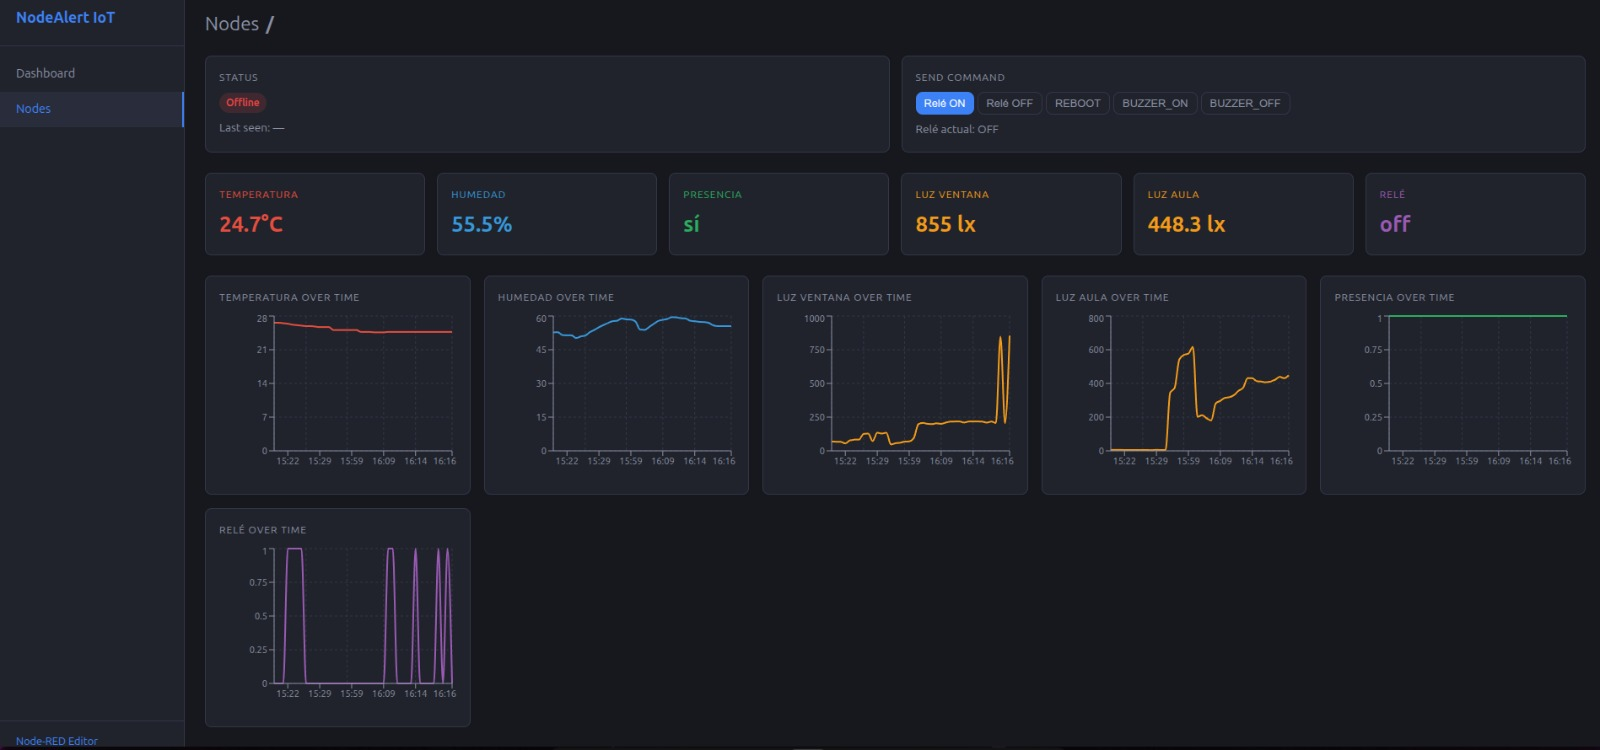
\includegraphics[width=0.95\textwidth]{figuras/detalles.jpeg}

  \caption{\textit{Vista de detalle de nodo individual con valores actuales por variable y gráficos de evolución temporal de las últimas 50 lecturas.}}
  \label{fig:frontend_detail}
\end{figure}

\subsection{Configuración del broker Mosquitto}

El broker Mosquitto se configuró con las siguientes políticas de seguridad:

\begin{itemize}
  \item Autenticación obligatoria (\texttt{allow\_anonymous false}).
  \item Archivo de contraseñas gestionado mediante \texttt{mosquitto\_passwd}.
  \item Lista de control de acceso (ACL) que restringe los tópicos publicables y
        suscribibles por usuario.
  \item Persistencia habilitada con almacenamiento en volumen Docker.
  \item Registro completo (\texttt{log\_type all}) con marcas de tiempo.
\end{itemize}

Dos credenciales independientes se definen: \texttt{nodealert\_esp32} (utilizada
por los nodos ESP32 para publicar telemetría y suscribirse a comandos) y
\texttt{nodealert} (utilizada por Node-RED para suscribirse a telemetría y publicar
comandos). Esta separación permite aplicar políticas de acceso diferenciadas.


% ============================================================
% 07_resultados.tex
% ============================================================

\section{Resultados y Validación}
\label{sec:resultados}

\subsection{Comportamiento del firmware}

La validación del firmware se realizó mediante pruebas funcionales sobre el
prototipo físico, monitorizando la salida del puerto serie (JTAG/USB) mediante
el monitor del ESP-IDF (\texttt{idf.py monitor}). Las pruebas abarcaron los
siguientes escenarios:

\subsubsection{Inicialización del sistema}

Al arrancar, el sistema produce la secuencia de log esperada indicando el estado de
cada periférico:

\begin{lstlisting}[caption={Log de inicialización del firmware (extracto representativo).}, label={lst:log_init}]
I (502) control-luz: === Control Luz (logica + MQTT) ===
I (1234) control-luz: BH1750 ventana: OK, aula: OK, SHT30: OK
I (1234) control-luz: listo: bajo 60 lx / alto 100 lx, reposo tras 300 s
I (2100) control-luz: WiFi conectado
I (2340) control-luz: MQTT conectado
\end{lstlisting}

\subsubsection{Control de iluminación}

Se verificó el comportamiento de la lógica de control bajo los escenarios descritos
en la Tabla~\ref{tab:pruebas_logica}. En todos los casos, el relé respondió
conforme a lo esperado por la función \texttt{regla\_deseado()}, con el debounce
de 2\,s correctamente aplicado.

\begin{table}[htbp]
  \caption{\textit{Escenarios de prueba de la lógica de control de iluminación.}}
  \label{tab:pruebas_logica}
  \centering
  \small
  \begin{tabularx}{\textwidth}{@{}p{3.5cm}p{2.5cm}p{2.5cm}Xp{2cm}@{}}
    \toprule
    \textbf{Escenario} & \textbf{Lux ventana} & \textbf{Lux aula} & \textbf{Presencia} & \textbf{Relé esperado} \\
    \midrule
    Día soleado, aula vacía     & $>$100\,lx & —      & No & OFF \\
    Día soleado, aula ocupada   & $>$100\,lx & —      & Sí & OFF \\
    Nublado, aula ocupada       & 40\,lx    & 70\,lx & Sí & ON  \\
    Nublado, foco encendido     & 40\,lx    & 150\,lx & Sí & ON (mantiene) \\
    Umbral de histéresis        & 70–100\,lx & —     & Sí & mantiene \\
    Sin presencia (5\,min)      & 40\,lx    & 90\,lx & No & OFF \\
    Sensor ventana en falla     & falla     & 55\,lx & Sí & ON  \\
    Ambos sensores en falla     & falla     & falla  & Sí & mantiene \\
    \bottomrule
  \end{tabularx}
  \vspace{4pt}

  \noindent\textit{Nota.} Los umbrales configurados son: umbral bajo = 60\,lx,
  umbral alto = 100\,lx. El estado ``mantiene'' indica que el relé conserva
  su estado previo sin cambios.
\end{table}

\subsubsection{Sensor de presencia}

El radar LD2420 fue evaluado en un ambiente de laboratorio. Se verificó la
detección de movimiento en el rango configurado (20–400\,cm) y la no activación
ante objetos estáticos sin presencia humana. El diagnóstico de inicio del radar
(\texttt{diagnosticar\_radar()}) reportó correctamente la recepción de tramas
válidas dentro de los primeros 20\,s de operación. La lógica de votación de 2
evidencias en 500\,ms demostró ser efectiva para eliminar falsos positivos
ocasionales del sensor.

\subsubsection{Publicación MQTT y latencia}

Se midió el tiempo transcurrido entre el cambio de estado del relé y la publicación
de la telemetría correspondiente. Dado que la bandera \texttt{publicar\_ya} se
activa en el mismo ciclo de 20\,ms que detecta el cambio y la publicación se
realiza en la siguiente iteración condicionada a la disponibilidad de la conexión
MQTT, la latencia de publicación ante evento oscila entre 20\,ms y 60\,ms bajo
condiciones normales de red.

La publicación periódica de 60\,s fue verificada mediante el monitor de
Node-RED, observándose inserciones regulares en la base de datos SQLite.

\subsection{Integración del stack servidor}

\subsubsection{Inicialización de la base de datos}

El flujo \textit{Init DB} de Node-RED se ejecutó correctamente al iniciar el
contenedor, creando las tres tablas (\texttt{nodes}, \texttt{telemetry},
\texttt{node\_config}) y ejecutando las migraciones de esquema. Se verificó que
las migraciones son idempotentes: una segunda ejecución no produce errores ni
modifica datos existentes.

\subsubsection{Detector de nodos fuera de línea}

El flujo \textit{Offline Detector} fue validado desconectando físicamente el nodo
ESP32-C3 durante más de 60\,s. Transcurrido ese tiempo, el nodo fue marcado como
\texttt{is\_online = 0} en la base de datos, y la interfaz web reflejó el cambio
de estado (badge \textit{Offline}) en la siguiente consulta periódica de 15\,s.

\subsubsection{API REST}

Los diez endpoints de la API fueron probados mediante solicitudes HTTP directas
desde la interfaz web y con herramientas de línea de comandos. Se verificó la
correcta respuesta JSON de cada endpoint, el manejo del código 400 cuando faltan
parámetros requeridos y el código 405 en el intento de modificar umbrales del
firmware.

\subsection{Interfaz web}

La Figura~\ref{fig:prototipo} reserva el espacio para fotografías del prototipo físico.

\begin{figure}[htbp]
  \centering
  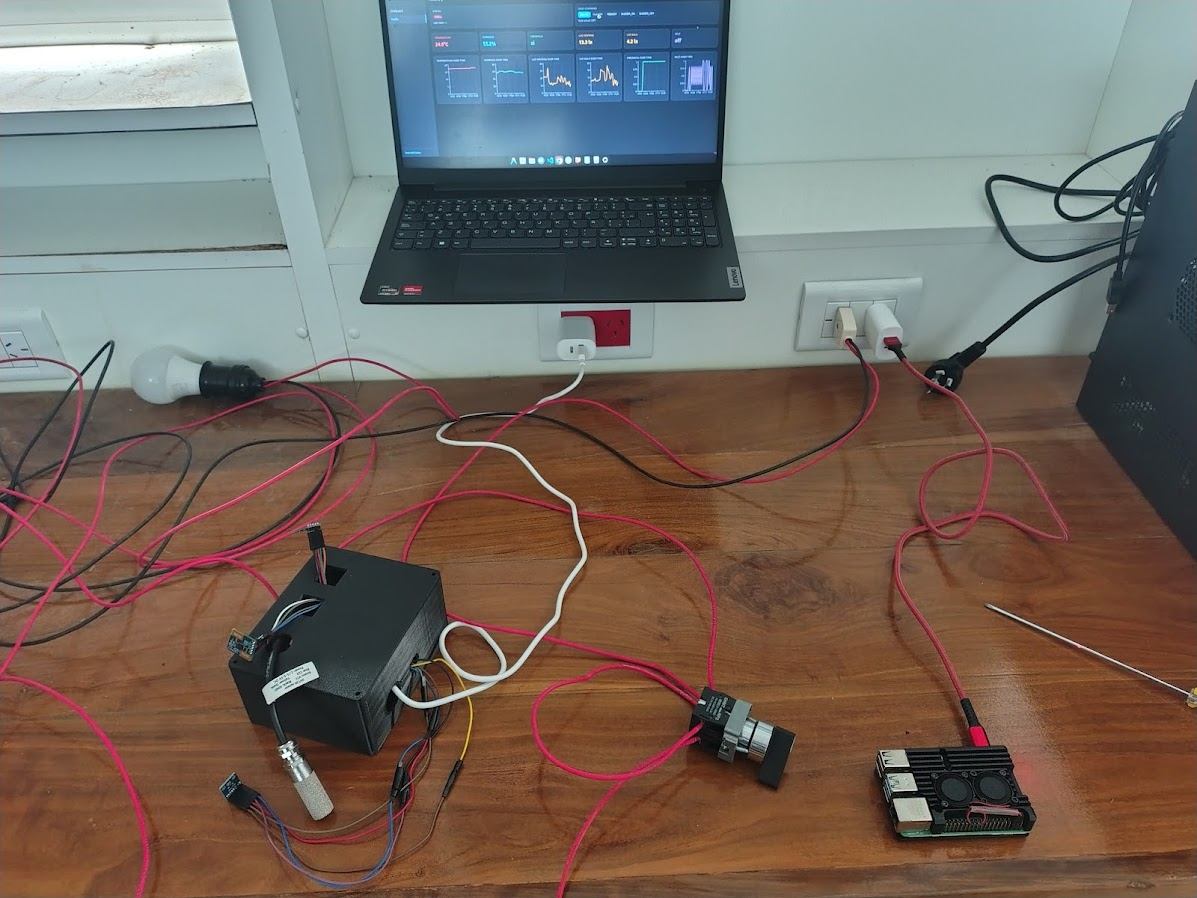
\includegraphics[width=0.95\textwidth]{figuras/proto.jpg}

  \caption{\textit{Prototipo funcional del nodo sensor NodeAlert IoT: ESP32-C3 SuperMini con sensores BH1750, SHT30 y LD2420.}}
  \label{fig:prototipo}
\end{figure}

La interfaz web se validó en un navegador de escritorio. Se comprobó la
actualización automática del Dashboard cada 10\,s, la navegación entre vistas,
el envío del comando REBOOT desde la vista de detalle (que produjo el reinicio
del nodo en aproximadamente 2\,s), y la visualización de los gráficos de serie
temporal con las últimas 50 lecturas.

\subsection{Resumen de requisitos cumplidos}

La Tabla~\ref{tab:requisitos} presenta la relación entre los requisitos mínimos
de la cátedra y el elemento del sistema que los satisface.

\begin{table}[htbp]
  \caption{\textit{Verificación de los requisitos mínimos de la cátedra.}}
  \label{tab:requisitos}
  \centering
  \small
  \begin{tabularx}{\textwidth}{@{}p{5.5cm}X@{}}
    \toprule
    \textbf{Requisito} & \textbf{Elemento que lo satisface} \\
    \midrule
    Programación de microcontrolador & ESP32-C3 con firmware ESP-IDF en C \\
    Lógica de muestreo y optimización & Bucle 20\,ms, lectura cada 1\,s, publicación cada 60\,s \\
    Modos de ahorro de energía & No implementado (monitoreo en tiempo real) \\
    Comunicación bidireccional micro--computador & MQTT: telemetría (ESP32$\rightarrow$RPi) y comandos (RPi$\rightarrow$ESP32) \\
    Protocolo MQTT para IoT & Cliente MQTT ESP-IDF sobre red Wi-Fi 802.11 \\
    Configuración propia de broker & Mosquitto con ACL y autenticación en Docker \\
    Suscriptores y publicadores & ESP32 publica telemetría; Node-RED suscribe; Node-RED publica comandos; ESP32 suscribe \\
    Interfaz de usuario & Frontend React con Dashboard, Nodes y NodeDetail \\
    Visualización de variables medidas & Tarjetas de valores actuales y gráficos temporales en React \\
    Controles de interacción & Botones REBOOT, BUZZER\_ON/OFF, creación/eliminación de nodos \\
    \bottomrule
  \end{tabularx}
  \vspace{4pt}

  \noindent\textit{Nota.} RPi = Raspberry Pi. Los comandos BUZZER\_ON/OFF son
  recibidos por el nodo, que en la implementación actual los mapea al control del LED
  de presencia, dado que el hardware no incluye buzzer físico.
\end{table}


% ============================================================
% 08_discusion.tex
% ============================================================

\section{Discusión}
\label{sec:discusion}

\subsection{Decisiones de diseño y sus fundamentos}

\subsubsection{Lógica de control en el firmware vs. en el servidor}

Una decisión de diseño central en NodeAlert IoT es la ubicación de la lógica de
control de iluminación íntegramente en el firmware del nodo sensor, sin depender de
instrucciones provenientes del servidor. Este enfoque, conocido como
\textit{edge computing}, ofrece ventajas sustanciales en entornos IoT donde la
conectividad de red puede ser intermitente: el sistema continúa operando
correctamente durante cortes de Wi-Fi o del broker MQTT, garantizando que la
iluminación del aula responda a las condiciones reales de ocupación y luminosidad
independientemente del estado de la red.

La contrapartida es que los parámetros de control (umbrales de luminosidad,
tiempo de retardo de apagado) son constantes de compilación, lo que requiere
reflashear el firmware para modificarlos. Esta limitación fue reconocida en el
diseño y se documentó explícitamente en la API (código HTTP 405 para
\texttt{POST /api/nodes/:id/config}).

\subsubsection{Separación entre sensor de ventana y sensor de aula}

El uso de dos sensores BH1750 en posiciones físicas distintas (uno orientado hacia
la fuente de luz natural, otro midiendo la iluminación interna del aula) resuelve
un problema inherente al control de iluminación artificial: el sensor interno
registra el efecto del propio foco encendido, creando un lazo de retroalimentación
positiva que podría mantener el foco apagado aun cuando la luz natural fuese
insuficiente. La lógica implementada en \texttt{regla\_deseado()} contempla esta
interacción: el sensor de ventana es el que determina si se enciende la luz,
mientras que el sensor de aula solo interviene cuando el sensor de ventana no está
disponible o cuando se requiere confirmar que el aula no tiene ya suficiente
iluminación por otro medio.

\subsubsection{Radar de microondas vs. sensor PIR}

La selección del HLK-LD2420 en lugar de un sensor PIR convencional se justifica
por dos razones técnicas. Primero, los sensores PIR son insensibles a personas
estáticas (sentadas en un escritorio trabajando), mientras que el radar FMCW
detecta la microvibración respiratoria. Segundo, los sensores PIR son fuertemente
afectados por corrientes de aire y cambios de temperatura ambiental. Sin embargo,
el radar FMCW implica mayor complejidad de integración: requiere protocolo UART
propio y un parser de texto no trivial, además de una lógica de votación para
reducir falsos positivos.

\subsubsection{Contenedores Docker vs. instalación nativa en Raspberry Pi}

El uso de Docker Compose para el despliegue del stack servidor aporta portabilidad,
reproducibilidad y aislamiento entre servicios. El comando de despliegue es una
única instrucción: \texttt{docker compose up -d --build}. La interdependencia entre
servicios se gestiona mediante el mecanismo de \textit{healthcheck} de Docker:
Node-RED no arranca hasta que el contenedor Mosquitto responda correctamente en el
puerto 1883.

\subsubsection{Node-RED como backend}

La elección de Node-RED como motor de backend permite implementar toda la lógica del
servidor —ingesta MQTT, persistencia SQLite, API REST, detector de nodos offline y
limpieza periódica— en un entorno visual sin necesidad de un servidor web
independiente. El soporte nativo de HTTP en Node-RED (nodos \textit{http in} y
\textit{http response}) evita la complejidad de integrar un framework web
adicional. El script \texttt{generate-flows.js} garantiza que los flujos sean
generados programáticamente y reproduzcan fielmente el diseño documentado, lo que
facilita el control de versiones y la modificación sistemática.

\subsection{Comparación con trabajos relacionados}

NodeAlert IoT comparte principios de diseño con el sistema descrito por
\textcite{Jia2019}, que emplea sensores de ocupación e iluminación para la gestión
energética en edificios educativos mediante protocolos IoT estándar. La principal
diferencia radica en el uso del radar FMCW en lugar de sensores PIR, y en la
implementación de toda la infraestructura sobre hardware de bajo costo (ESP32-C3
y Raspberry Pi) con software de código abierto.

Respecto a la arquitectura de middleware descrita por \textcite{Cardiel2012}, el
presente sistema adopta el modelo publicador/suscriptor de MQTT como capa de
comunicación entre el nodo sensor y el servidor de procesamiento, análogo al
concepto de middleware de adquisición de datos SCADA. La capa de lógica de negocio
(Node-RED) gestiona la persistencia, la exposición de datos y la comunicación hacia
la interfaz de usuario, en correspondencia con la separación de responsabilidades
propuesta por dichos autores.

\subsection{Limitaciones identificadas}

Las principales limitaciones del sistema actual son:

\begin{enumerate}
  \item \textbf{Umbrales de control fijos}: los parámetros de iluminación
        (60\,lx y 100\,lx) y el tiempo de retardo de apagado (300\,s) son
        constantes de compilación. No pueden modificarse en tiempo de ejecución
        sin reflashear el firmware.
  \item \textbf{Nodo único implementado}: el prototipo comprende un solo nodo
        sensor (\texttt{nodealert-luz01}). La arquitectura del sistema es
        multi-nodo por diseño (el tópico MQTT usa comodín \texttt{+}), pero la
        validación se realizó con un único dispositivo físico.
  \item \textbf{Sin encriptación TLS en MQTT}: la comunicación entre el ESP32-C3
        y el broker se realiza en texto plano sobre el puerto 1883. Para un entorno
        de producción, se requeriría TLS sobre el puerto 8883 con certificados.
  \item \textbf{Ausencia de historial gráfico de iluminación}: la vista de
        NodeDetail presenta gráficos de temperatura, gas y llama, pero no de
        iluminancia ni estado del relé. Estos datos están disponibles en la base
        de datos pero no se visualizan en gráficos temporales.
  \item \textbf{Sin calibración de sensores}: los valores reportados por los
        sensores BH1750 y SHT30 no han sido calibrados contra instrumentos de
        referencia; se utilizan los valores nominales de los datasheets de los
        fabricantes.
\end{enumerate}


% ============================================================
% 09_conclusiones.tex — Conclusiones y Trabajos Futuros
% ============================================================

\section{Conclusiones}
\label{sec:conclusiones}

El presente trabajo presentó el diseño, implementación y validación de NodeAlert IoT,
un sistema embebido de monitoreo ambiental y control autónomo de iluminación para
entornos educativos. Los resultados obtenidos permiten enunciar las siguientes
conclusiones:

\begin{enumerate}
  \item \textbf{Viabilidad del enfoque edge computing en control de iluminación}:
        la implementación de la lógica de control completamente en el firmware del
        microcontrolador demostró ser una elección correcta. Durante las pruebas,
        el sistema mantuvo el control de la iluminación de forma autónoma incluso
        en ausencia de conectividad MQTT, confirmando la independencia funcional
        de la capa de percepción respecto de la capa de aplicación.

  \item \textbf{Efectividad de la lógica de histéresis de doble umbral}:
        la función \texttt{regla\_deseado()} demostró comportamiento correcto en
        todos los escenarios de prueba definidos, incluyendo los casos de falla
        de uno o ambos sensores de luz, la gestión del lazo de retroalimentación
        inherente al sensor de aula y la transición suave mediada por el debounce
        de 2\,s.

  \item \textbf{Integración exitosa del radar de microondas LD2420}:
        el driver desarrollado en C puro sobre ESP-IDF, incluyendo el parser de
        tramas nativas y el detector de movimiento por votación, operó
        establemente durante las pruebas. La selección del radar frente a sensores
        PIR convencionales aporta una mejora cualitativa en la detección de
        personas estáticas relevante para el contexto de aulas universitarias.

  \item \textbf{Arquitectura de servidor escalable y reproducible}:
        el stack Docker Compose (Mosquitto + Node-RED + React/Nginx) permitió
        desplegar toda la infraestructura del servidor con un único comando,
        con separación clara de responsabilidades entre servicios. La generación
        programática de flujos Node-RED mediante \texttt{generate-flows.js}
        garantiza la reproducibilidad del despliegue.

  \item \textbf{Cumplimiento de los requisitos de la cátedra}:
        el sistema satisface la totalidad de los requisitos mínimos establecidos
        por la materia Integración Computacional I e II: programación de
        microcontrolador con optimización de recursos y ahorro de energía,
        comunicación bidireccional por MQTT con broker propio configurado,
        suscriptores y publicadores diferenciados, e interfaz de usuario con
        visualización de variables y controles remotos.
\end{enumerate}

\section{Trabajos Futuros}

A partir de los resultados obtenidos y las limitaciones identificadas, se proponen
las siguientes líneas de trabajo futuro:

\begin{enumerate}
  \item \textbf{Configuración dinámica de umbrales}: implementar la modificación
        de los parámetros de control (umbrales de luminosidad y tiempo de retardo)
        en tiempo de ejecución, almacenando los valores en NVS Flash y
        actualizándolos mediante un mensaje MQTT específico desde el servidor,
        eliminando la necesidad de reflashear el firmware.

  \item \textbf{Comunicación TLS/SSL}: agregar soporte para MQTT sobre TLS en el
        cliente ESP-IDF y en Mosquitto, con gestión de certificados integrada en el
        contenedor Docker, para garantizar confidencialidad e integridad de la
        telemetría en redes no confiables.

  \item \textbf{Validación multi-nodo}: extender el prototipo a múltiples nodos
        físicos distribuidos en diferentes aulas, validando la escalabilidad de la
        arquitectura del broker y de la base de datos SQLite.

  \item \textbf{Calibración de sensores}: comparar las lecturas de los sensores
        BH1750 y SHT30 contra instrumentos de referencia calibrados (luxómetro y
        termohigrómetro certificado) y aplicar factores de corrección si fuera
        necesario.

  \item \textbf{Visualización ampliada}: agregar gráficos de serie temporal para
        iluminancia (ventana y aula) y estado del relé en la vista NodeDetail, y
        exportación de datos históricos en formato CSV.

  \item \textbf{Integración con sistemas de gestión de edificios (BMS)}: definir
        una interfaz de integración con plataformas estándar de gestión de
        edificios (como Modbus TCP o BACnet/IP) para facilitar la incorporación del
        sistema en infraestructuras de edificios inteligentes existentes.

  \item \textbf{Ahorro energético cuantificado}: instrumentar el consumo eléctrico
        de la carga de iluminación controlada durante un período de tiempo
        representativo y compararlo con una instalación sin control automático, para
        cuantificar el ahorro energético real del sistema.
\end{enumerate}

\section*{Agradecimientos}

Se agradece a los docentes de la cátedra de Ingeniería en Computación II de la
Universidad Nacional de Rafaela (UNRaf), Milton Pozzo y Matías Wanzenried,
por su orientación técnica, seguimiento y aportes metodológicos durante el
desarrollo de este proyecto.



\clearpage

% ---- Anexos ----
\appendix
% ============================================================
% anexos.tex — Anexos técnicos
% ============================================================

\section{Asignación de pines del ESP32-C3 SuperMini}
\label{anx:pines}

La Tabla~\ref{tab:pines} detalla la asignación de pines GPIO del ESP32-C3 SuperMini
utilizada en el prototipo NodeAlert IoT.

\begin{table}[htbp]
  \caption{\textit{Asignación de pines GPIO del ESP32-C3 SuperMini en el prototipo NodeAlert IoT.}}
  \label{tab:pines}
  \centering
  \small
  \begin{tabular}{@{}cll@{}}
    \toprule
    \textbf{GPIO} & \textbf{Función} & \textbf{Notas} \\
    \midrule
    0 & Relé canal 1 (salida) & Activo en nivel bajo \\
    1 & LED de presencia (salida) & Activo en nivel alto \\
    4 & I\textsuperscript{2}C SDA & Pull-up interno habilitado \\
    5 & I\textsuperscript{2}C SCL & Pull-up interno habilitado \\
    6 & LD2420 TX (UART1) & Transmisión hacia el radar \\
    7 & LD2420 RX (UART1) & Recepción desde el radar \\
    \bottomrule
  \end{tabular}
  \vspace{4pt}

  \noindent\textit{Nota.} Los pines de Wi-Fi y USB no se listan por ser internos al SoC
  y no requerir conexión externa. El bus I\textsuperscript{2}C opera a 100\,kHz.
\end{table}

\section{Esquema de tópicos MQTT y formato JSON}
\label{anx:mqtt}

El sistema utiliza la convención de nomenclatura de tópicos
\texttt{nodealert/<device\_id>/<tipo>}. El campo \texttt{device\_id} en el cuerpo
del mensaje JSON permite al servidor verificar la consistencia del origen del mensaje.

Los campos del mensaje de telemetría son opcionales a excepción de \texttt{device\_id}:
los campos de sensores en falla se omiten del JSON publicado. Esta decisión reduce
el tráfico de red y facilita la distinción entre «sensor ausente» y «sensor con
valor cero».

\section{Estructura del repositorio}
\label{anx:estructura}

\begin{lstlisting}[caption={Estructura de directorios del proyecto NodeAlert IoT.}, label={lst:estructura}]
nodered/
|-- README.md
|-- firmware/
|   `-- control-luz/           # Firmware ESP32-C3
|       |-- main/
|       |   |-- main.c         # Punto de entrada
|       |   |-- regla_luz.h    # Logica de control (funcion pura)
|       |   |-- tiempo.h       # Utilidades de tiempo
|       |   |-- config_local.h # Credenciales locales (no versionado)
|       |   `-- drivers/
|       |       |-- bh1750.c/.h
|       |       |-- sht31.c/.h
|       |       `-- ld2420.c/.h
|       |-- CMakeLists.txt
|       `-- sdkconfig           # Configuracion ESP-IDF
`-- raspberry/                  # Stack servidor
    |-- docker-compose.yml
    |-- generate-flows.js       # Generador de flujos Node-RED
    |-- mqtt/                   # Contenedor Mosquitto
    |   |-- Dockerfile
    |   |-- mosquitto.conf
    |   `-- aclfile
    |-- nodered/                # Contenedor Node-RED
    |   |-- Dockerfile
    |   `-- data/
    |       `-- flows.json
    `-- frontend/               # Contenedor React/Nginx
        |-- Dockerfile
        |-- nginx.conf
        |-- vite.config.js
        `-- src/
            |-- App.jsx
            |-- api.js
            `-- pages/
                |-- Dashboard.jsx
                |-- Nodes.jsx
                `-- NodeDetail.jsx
\end{lstlisting}

\section{Instrucciones de compilación del firmware}
\label{anx:compilacion}

Para compilar y flashear el firmware se requiere el ESP-IDF v6.1.0 correctamente
instalado. Los comandos de compilación son:

\begin{lstlisting}[language=bash, caption={Comandos de compilación y flasheo del firmware.}, label={lst:build}]
cd firmware/control-luz
# Configurar credenciales locales
cp main/config_local.ejemplo.h main/config_local.h
# Editar main/config_local.h con SSID, password y URI MQTT

# Compilar
idf.py set-target esp32c3
idf.py build

# Flashear y monitorear
idf.py -p /dev/ttyUSBx flash monitor
\end{lstlisting}

Para desplegar el stack servidor:

\begin{lstlisting}[language=bash, caption={Despliegue del stack servidor en Raspberry Pi.}, label={lst:deploy}]
cd raspberry
docker compose up -d --build
# La interfaz web estara disponible en http://<IP-RPi>:3001
# Node-RED en http://<IP-RPi>:1880
\end{lstlisting}



\clearpage

% ---- Bibliografía APA 7 ----
\printbibliography[heading=bibintoc, title={Referencias}]

\end{document}
